\documentclass[12pt]{article}

% Ћирилица: кодирање фонта и језик (српски, ћирилица)
\usepackage[T2A]{fontenc}
\usepackage[utf8]{inputenc}
\usepackage[serbianc]{babel}

% Величина стране и маргине
\usepackage[a4paper,top=2cm,bottom=2cm,left=2.5cm,right=2.5cm]{geometry}

% Корисни пакети
\usepackage{amsmath}
\usepackage{enumitem}
\usepackage{float}
\usepackage{booktabs}
\usepackage{tcolorbox}
\tcbuselibrary{breakable}
\usepackage[colorlinks=true, allcolors=blue]{hyperref}

% Цртање електричних кола (европски симболи)
\usepackage[european]{circuitikz}
\usetikzlibrary{babel}

% Оквир за решене примере
\newtcolorbox[auto counter]{primer}{breakable,
    colback=white, colframe=black!55, colbacktitle=black!55, coltitle=white,
    fonttitle=\bfseries\small, title={Пример~\thetcbcounter},
    boxrule=0.5pt, arc=1.5pt, left=6pt, right=6pt, top=3pt, bottom=3pt,
    before skip=8pt, after skip=10pt}

% Оквир за кључне формуле
\newtcolorbox{kljucno}{colback=blue!4, colframe=blue!45!black,
    boxrule=0.5pt, arc=1.5pt, left=8pt, right=8pt, top=4pt, bottom=4pt}

\title{Mono - Jetronic систем убризгавања - пропитивање}
\author{Аутоелектронски системи 2}
\date{}

\begin{document}
\maketitle

%##################################################################
\section{Mono-Jetronic}
%##################################################################

За разлику од KE-Jetronic и L-Jetronic система, овај систем има \textbf{централно}
убризгавање. Централни колектор равномерно распоређује гориво према појединим
цилиндрима и његова највећа примена је у четвороцилиндричним моторима.

Потребне информације о раду мотора се прикупљају помоћу сензора и даље се обрађују
у ЕУЈ (електронска управљачка јединица). На основу свих информација
израђују се управљачки сигнали за \textbf{вентил убризгавања, корачни мотор за
регулацију празног хода и вентил утрошка бензинских испарења}.

Код KE и L-Jetronic система свака бризгаљка убризгава гориво испред усисног
вентила свог цилиндра (убризгавање у више тачака, MPI). Mono-Jetronic има само
\textbf{једну бризгаљку}, смештену у централној јединици изнад пригушног
лептира, на самом почетку усисне цеви (убризгавање у једној тачки, SPI).
Бризгаљка је електромагнетни вентил, а количину горива одређује управљачка
јединица дужином импулса, тј. временом за које држи бризгаљку отвореном.
Гориво се затим, заједно са ваздухом, кроз усисни колектор разводи до свих
цилиндара.

\begin{figure}[H]
    \centering
    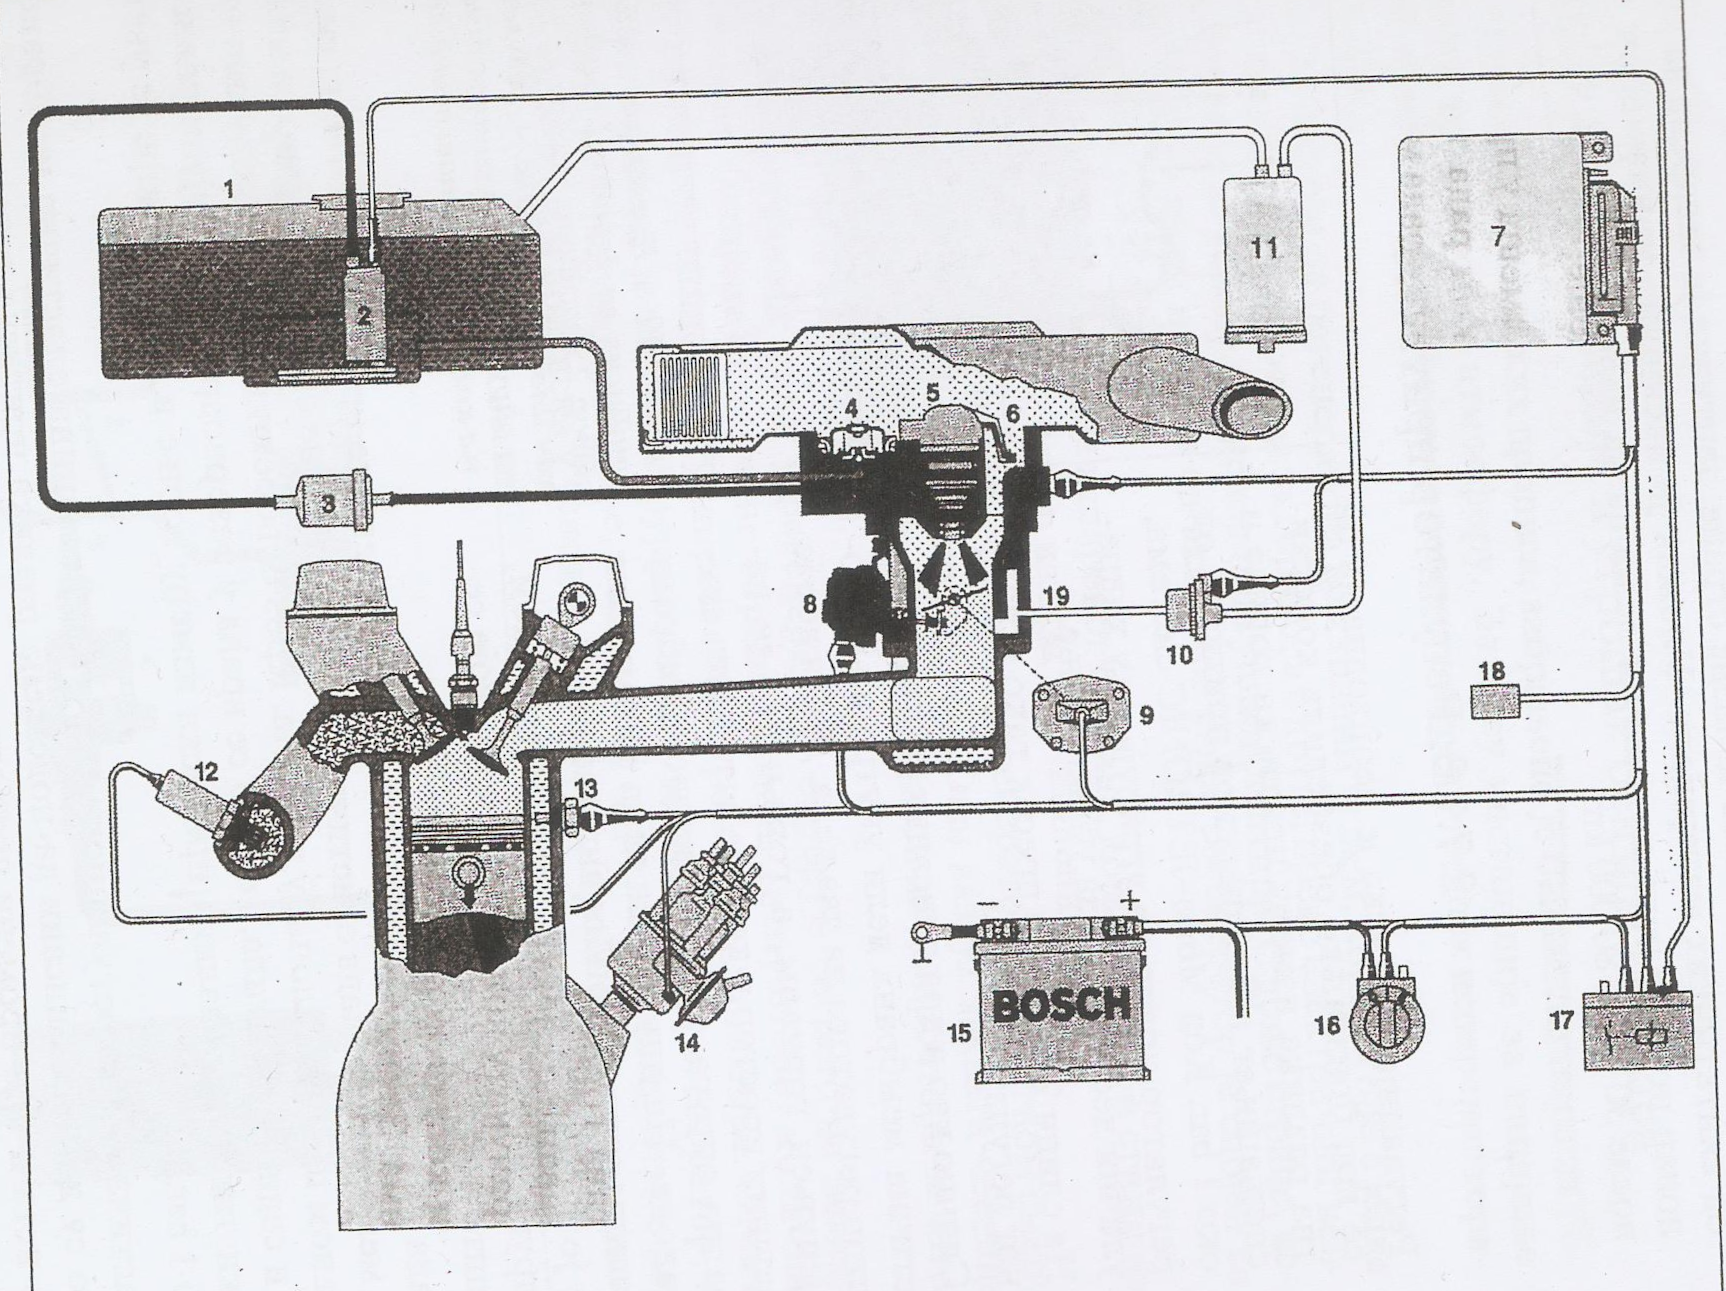
\includegraphics[width=0.7\textwidth]{slike/Mono.png}
    \caption{Основна шема Mono-Jetronic система убризгавања}
    \label{fig:mono-sema}
\end{figure}

\begin{kljucno}

      \begin{enumerate}[noitemsep]
    \item[1.] Резервоар за гориво
    \item[2.] Електрична пумпа
    \item[3.] Филтер за гориво
    \item[4.] Регулатор притиска
    \item[5.] Електромагнетна бризгаљка
    \item[6.] Сензор температуре усисаног ваздуха
    \item[7.] Електронска управљачка јединица
    \item[8.] Корачни (степ) мотор
    \item[9.] Потенциометар пригушног лептира
    \item[10.] Вентил за регенерисано гориво (EVAP)
    \item[11.] Регенератор са активним угљем
    \item[12.] ЛАМБДА сонда
    \item[13.] Сензор температуре мотора
    \item[14.] Разводник паљења
    \item[15.] Акумулатор
    \item[16.] Контакт-кључ
    \item[17.] Електронски релеј
    \item[18.] Прикључак за дијагностику
    \item[19.] Уређај за убризгавање (централна јединица)
\end{enumerate}
      
\end{kljucno}

\section{Шта решава и по коју цену}

KE и L-Jetronic су прецизни, али скупи системи: имају по једну бризгаљку за сваки
цилиндар, мерач протока ваздуха, систем под високим притиском и много
механичких или електронских делова. За мале и јефтине аутомобиле то је било
прескупо, а карбуратор више није могао да испуни строге прописе о издувним
гасовима, нарочито уз катализатор, који тражи смешу са $\lambda \approx 1$.

Mono-Jetronic је настао као \textbf{јефтина замена за карбуратор}, која задржава
главне предности електронског убризгавања:

\begin{itemize}[noitemsep]
    \item \textbf{једна бризгаљка} уместо четири, и централна јединица која се
          уграђује на место карбуратора, па се мотор мало мења,
    \item \textbf{низак притисак горива} (око 1~bar), па су пумпа, водови и
          регулатор једноставнији и јефтинији,
    \item \textbf{нема мерача протока ваздуха}: количина ваздуха се израчунава
          посредно, из угла пригушног лептира и броја обртаја,
    \item електронска регулација са ЛАМБДА сондом, па систем ради са
          трокомпонентним катализатором и испуњава прописе.
\end{itemize}

\textbf{Цена} тих уштеда је мања прецизност. Гориво путује од бризгаљке до
цилиндара кроз цео усисни колектор, па:

\begin{itemize}[noitemsep]
    \item део горива се таложи на зидовима колектора као филм, па смеша није
          иста у свим цилиндрима, нарочито код хладног мотора,
    \item при наглим променама оптерећења смеша касни за потребама мотора, па
          су потребне посебне корекције,
    \item посредно мерење ваздуха мање је тачно од мерача протока, па систем
          мора стално да се прилагођава (адаптација),
    \item снага и економичност мотора су нешто мањи него са убризгавањем у
          више тачака.
\end{itemize}

Због тога се Mono-Jetronic највише користио код мањих четвороцилиндричних
мотора, где су ниска цена и испуњење еколошких прописа били важнији од највеће
снаге.

\section{Шта је додато или промењено у односу на KE и L-Jetronic}

\begin{table}[H]
    \centering
    \small
    \renewcommand{\arraystretch}{1.3}
    \begin{tabular}{p{4.2cm} p{4.6cm} p{4.6cm}}
        \toprule
                                & \textbf{KE / L-Jetronic}               & \textbf{Mono-Jetronic} \\
        \midrule
        бризгаљке               & по једна за сваки цилиндар              & једна, централна \\
        место убризгавања       & испред усисних вентила                  & изнад пригушног лептира \\
        притисак горива         & око 2,5--5~bar                          & око 1~bar \\
        мерење ваздуха          & мерна плоча / заклопка                  & нема мерача, рачуна се из $\alpha$ и $n$ \\
        пригушни лептир         & прекидач лептира                        & потенциометар са две отпорне траке \\
        празан ход              & биметални вентил / регулатор празног хода & корачни мотор помера лептир \\
        хладан старт            & бризгаљка за хладан старт               & продужење импулса главне бризгаљке \\
        пумпа                   & у водовима (in-line)                    & у резервоару (in-tank) \\
        \bottomrule
    \end{tabular}
    \caption{Најважније разлике у односу на KE и L-Jetronic}
\end{table}


\subsection{Регенерација и утрошак бензинских пара}

Прописи забрањују испуштање бензинских пара из резервоара у атмосферу. Зато
су инсталације опремљене уређајем за регенерацију и утрошак тих пара. Уређај чине \textbf{регенератор са активним угљем} и електрични
\textbf{EVAP вентил}. Регенератор је са једне стране спојен са резервоаром, а
са друге, преко EVAP вентила, са усисном цеви испод пригушног лептира. Доња
страна регенератора има отвор ка атмосфери.

Активни угаљ упија честице бензинских пара из резервоара. Када EVAP вентил
отвори пролаз, потпритисак у усисној цеви повлачи свеж ваздух кроз
регенератор у супротном смеру. Ваздух понесе упијено гориво и одводи га у
цилиндре, где сагори, а угаљ се тиме чисти за ново упијање.

\begin{figure}[H]
    \centering
    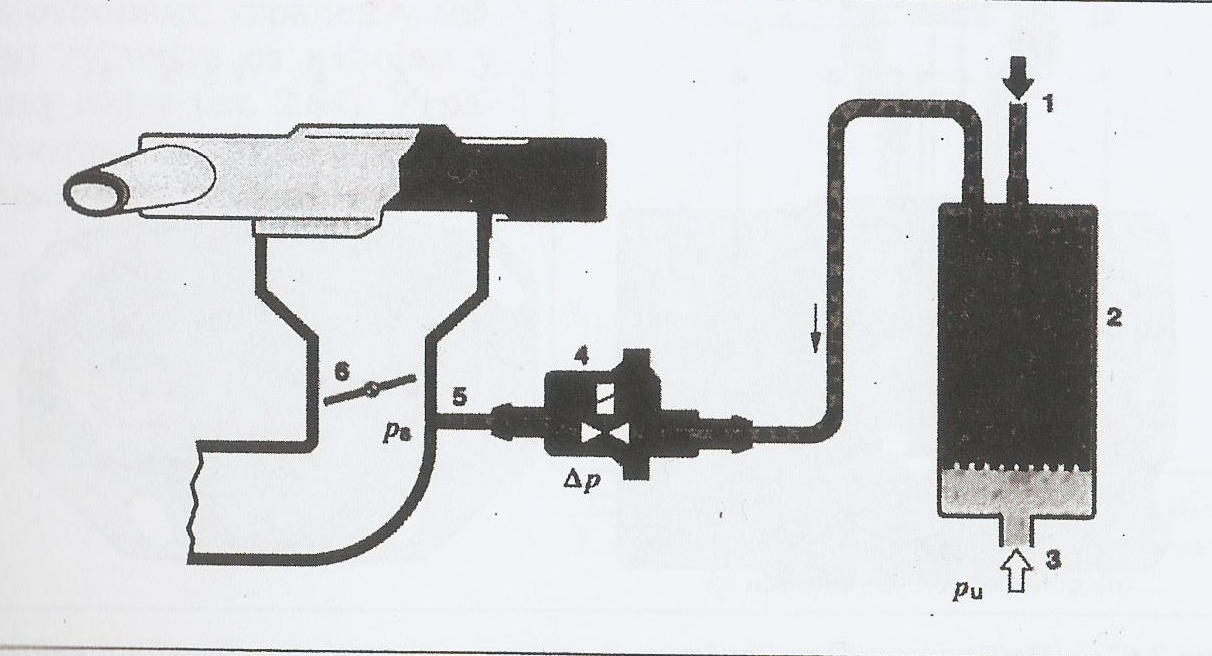
\includegraphics[width=0.4\textwidth]{slike/2.png}
    \caption{Регенерација и утрошак бензинских пара}
    \label{fig:mono-sema}
\end{figure}

Количина горива из регенератора зависи од разлике притисака, која је највећа
у празном ходу, када је регенератор пун горива. Тада би неконтролисано
доведено гориво пореметило смешу, а при пуном оптерећењу је обрнуто: разлика
притисака је мала, па је и проток мали. Проблем решава EVAP вентил, чијим
отварањем управља електронска управљачка јединица, према програму и тренутном
режиму рада мотора.

\section{Електронска управљачка јединица}

Кућиште управљачке јединице је од полиамида, ојачаног стакленим влакнима, да би
електронски елементи били заштићени од механичких и термичких утицаја. Јединица
се најчешће смешта у путнички простор или у ниши испод ветробрана, где су мање
вибрације и температуре, а ретко у моторни простор.

Цела електроника налази се на једној штампаној плочи. Излазни степени и
стабилизатор напона постављени су на хладњак са ребрима. Јединица се преко
вишеполног утикача (25 полова) повезује са акумулатором, сензорима и
извршним органима.

\begin{figure}[H]
    \centering
    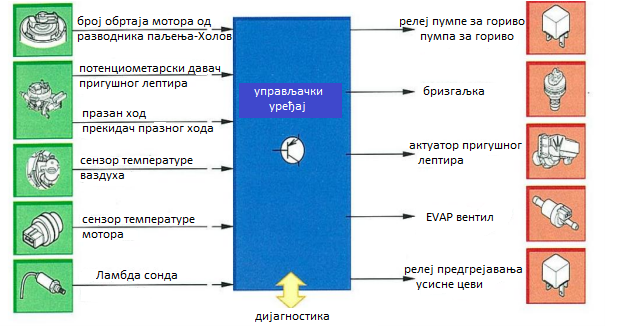
\includegraphics[width=0.7\textwidth]{slike/image1.png}
    \caption{Блок шема система}
    \label{fig:mono-sema}
\end{figure}

\begin{figure}[H]
    \centering
    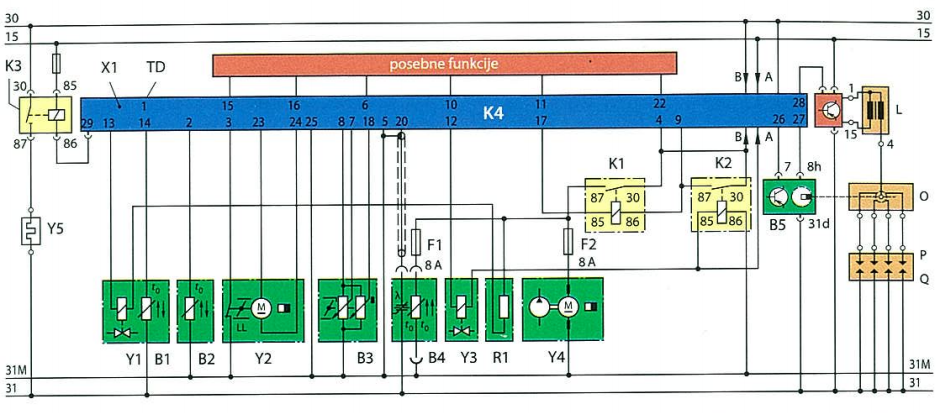
\includegraphics[width=0.9\textwidth]{slike/image2.png}
    \caption{Електрична шема система}
    \label{fig:mono-sema}
\end{figure}

\begin{itemize}[leftmargin=1.6cm, labelwidth=0.7 cm, labelsep=0.3cm, align=left, itemsep=0pt]
    \item[\textbf{В1}] сензор температуре ваздуха
    \item[\textbf{В2}] сензор температуре мотора
    \item[\textbf{В3}] потенциометар пригушног лептира
    \item[\textbf{В4}] ламбда сонда
    \item[\textbf{В5}] Холов сензор
    \item[\textbf{F1, F2}] осигурачи
    \item[\textbf{К1}] релеј пумпе горива
    \item[\textbf{К2}] главни релеј
    \item[\textbf{К3}] релеј за предгрејање усисног ваздуха
    \item[\textbf{К4}] управљачки уређај
    \item[\textbf{R1}] предотпорник
    \item[\textbf{Y1}] централна бризгаљка
    \item[\textbf{Y2}] регулатор пригушног лептира са прекидачем празног хода
    \item[\textbf{Y3}] EVAP вентил
    \item[\textbf{Y4}] пумпа за гориво
    \item[\textbf{Y5}] грејач усисног ваздуха
\end{itemize}

\begin{kljucno}
      \begin{itemize}
    \item Маса јединице изведена је преко два извода. Електронски део за пријем
          сигнала NTC отпорника, ЛАМБДА сонде и потенциометра има посебан спој
          са масом, а друга маса служи за извршне органе, кроз које теку веће
          струје.
    \item Веза са ЛАМБДА сондом изведена је оклопљеним (ширмованим) каблом,
          да би се избегле индуктивне сметње од других струјних кола.
    \item Пумпа за гориво напаја се преко посебног релеја, којим управља
          јединица. По укључењу контакт-кључа пумпа ради неколико секунди, да
          подигне притисак у систему (динамичко управљање пумпом). Ако мотор
          престане да ради, а контакт је и даље укључен (на пример после
          незгоде), релеј аутоматски прекида напајање пумпе.
\end{itemize}
\end{kljucno}

\section{Обрада података}

\begin{kljucno}
      Прикупљени подаци доводе се до управљачке јединице, која их прилагођава и
обрађује. Према уграђеном програму јединица израђује управљачке сигнале за
бризгаљку, корачни мотор лептира и EVAP вентил.
\end{kljucno}

\begin{kljucno}
      \begin{itemize}
    \item \textbf{Аналогно-дигитални претварач.} Аналогни сигнали (отпор
          потенциометра, напон ЛАМБДА сонде, напон давача температуре, напон
          акумулатора) претварају се у дигиталне, које микропроцесор може да
          обради. Сигнали броја обртаја из система паљења већ су импулси, па
          се обликују посебним колом.
    \item \textbf{Микропроцесор} прима податке од сензора преко интерфејса и
          А/Д претварача и, према програму, израчунава време убризгавања.
          Повезан је са меморијом \textbf{EPROM}, у којој су програм и
          подаци (кодови, дијаграми), и са меморијом \textbf{RAM}, у коју се
          уписују адаптивне корекције. Да се подаци не би изгубили после
          гашења мотора, RAM је стално повезан са акумулатором. Радну
          учестаност од 6~MHz даје кварцни осцилатор.
    \item \textbf{Излазни степени} су појачавачи са транзисторима снаге, преко
          којих микропроцесор управља бризгаљком, корачним мотором, EVAP
          вентилом, релејем пумпе и контролном лампицом.
\end{itemize}
\end{kljucno}

\section{Прилагођавање раду мотора}

Управљачка јединица прилагођава убризгавање следећим режимима и условима рада:
\begin{itemize}[noitemsep]
    \item хладан старт,
    \item загревање мотора,
    \item температура усисаног ваздуха,
    \item празан ход,
    \item пуно оптерећење,
    \item ограничење броја обртаја,
    \item кочење мотором,
    \item принудна вожња у случају квара,
    \item компензација у прелазним режимима,
    \item ЛАМБДА регулација,
    \item адаптација радне смеше,
    \item компензација пада напона.
\end{itemize}

\end{document}